\subsection{Convergence Detection}
We found that there is no convergence detection in U Kang's implementation of BP. The algorithm terminates after fixed number of iterations, without knowing whether it converging or not. One more map-reduce job might be added after each iteration to perform the convergence detection, which is a useful enhancement.

\subsection{Methods for Extending Fast BP to Multiclass Problems}

\subsubsection{Error Correcting Code Methods}

\subsubsection*{Motivation}
Fast BP is now limited to solve problems with only 2 labels. Formally extending Fast BP to multiclass can be difficult. Instead of formally formulating the multiclass Fast BP, we emphasize BP as a tool to give the correct label rather than compute the probability. Thus we can divide a single multiclass problem into several binary problems so that we can use Fast BP to give the label.


\subsubsection*{General Definition}

To solve a multiclass problem, which has $k$ classes and $l$ training example $(x_{1},y_{1})...(x_{l},y_{l})$, we can use error correcting code approach, which usually involves the following steps:

\subsubsection*{Code Design}

In this step, for each class in the $k$ classes, we design a unique $N$ bits code. For example, for a problem recognizing hand writings of 10 digits, we can define the following 6 bits error codes, shown in Figure 1.

\begin{figure}[!htbp]
\centering
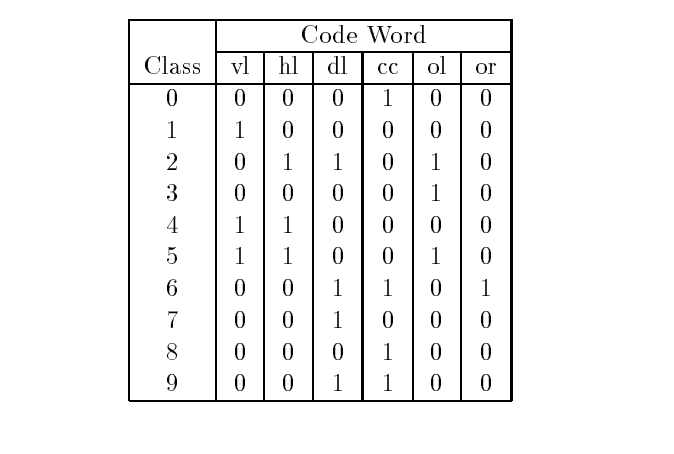
\includegraphics[bb=0 0 680 500,scale=.3]{FIG/code.png} 
\caption{Coding scheme for 10 digits recognizing problem}
\end{figure}

The meaning of those codes follows the description in the figure 2 from \cite{Thomas1995}.


\begin{figure}[!htbp]
\centering
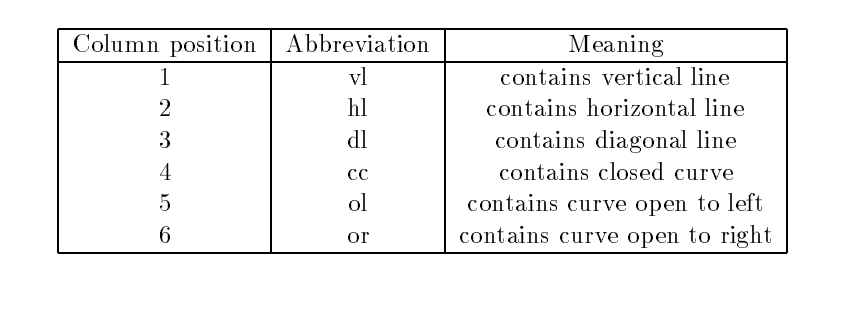
\includegraphics[bb=0 0 860 300,scale=.3]{FIG/meaning.png} 
\caption{Meaning of each bit}
\end{figure}
 
There are basically two principles for design a code\cite{Thomas1995}:
\begin{enumerate}
	\item \textbf{Row Distance}: The hamming distance between each two classes' codes should be as large as possible to make classes more distinguishable from each other.
	\item \textbf{Column Distance}: Each bit classifier should be independent from each other.
\end{enumerate}  

It is obvious that there is a trade-off between those two principles, which leads to different code design methods. We will adapt the one described in Thomas's Paper\cite{Thomas1995}, which is every effective to generate compact yet distinguish code. 

\subsubsection*{Running Fast BP for Bits}

As we already described in the previous sections, after designing of code, we run Fast BP for each bits, note as $f_{1}...f_{n}$. We can interpret $f_{i}(x)$ as the probability that the number appear on the $i^{th}$ bit of the code for a given example $x$ is 1.

\subsubsection*{Deciding Label}

For a node $r$, after computation, we get a vector of predictions of those functions:

\begin{gather*}
	f(r) = (f_{1}(r)...f_{n}(r)) 
\end{gather*}



In order to make final prediction we should find the class which is \textit{closest} to $f(r)$.

In general, there are different approaches to achieve this:

\begin{enumerate}
	\item \textbf{Hamming Decoding}: Transform $f(r)$ from real-value to binary value, and calculate the Hamming distance with code of each class. The label that has the shortest hamming distance is chosen.
	\item \textbf{Loss-based Decoding}: This method is introduced in \cite{Erin2000}, which defines a loss function between probability made by $f$ and the target bit of class, without transform $f(r)$ into binaries.
\end{enumerate}

\subsubsection*{Practical Scheme for too Many Labels}

Error Correcting Code is a powerful tool, but in a distributed environment, if the number of labels is large, it may be very expensive, because it requires to run Fast BP for every bit. So in order to make error correcting code more practical, we introduce the following two scheme:

\begin{enumerate}
	\item \textbf{One-Vs-All}: In this scheme every class is associated with a classifier that tells whether an incoming example is in this class or not. The final prediction is made according to some predefined decision value, like probability given by Logistics Regression.
	\item \textbf{All-Vs-All}: A classifier is trained for every pair of classes. As there are $O(n^{2})$ classifiers to train, some algorithms are introduced to reduce the number of classifier pairs\cite{Platt2000}
\end{enumerate}

Actually, the two schemes are just special case of ECOC, but are much more straight forward.

\subsubsection{Quadratic approximation for FaBP extension}
A significant fact of the original \textbf{FaBP} algorithm is the assumption that all parameters are ``about half'', i.e. close to 1/2. This assumption provides a foundation for the correctness of Maclaurin series expansion used in the analysis. However, when there are more than two classes, without the concept of odd-ratio, we cannot achieve the a similar assumption for any parameter. But we can use the quadratic approximation, i.e. second order Taylor approximation for the logarithms, i.e. instead of using $\log(x) \approx \log(1)+\log^{\prime}(1)(x-1)$ with the assumption that $x$ (the odd-ratio) is close to $\frac{1}{2}$, we use
$$\log(x)\approx \log(1)+\log^{\prime}(x-1)+\frac{\log^{\prime\prime}(1)}{2}(x-1)^2$$
without the ``about half'' assumption.

Take the original belief update rule $b_i(x_i) = \eta\cdot \phi_i(x_i)\cdot\Pi_{j\in N(i)}m_{ij}(x_i)$ for example, we can derive
\begin{equation}
\log(b_i(x_i))=\log\eta + \log(\phi_i(x_i))+ \sum_{j\in N(i)}\log(m_{ij}(x_i))
\end{equation}
\begin{equation}
\label{eq:quadratic approx}
2b_i(x_i)-\frac{1}{2}b_i^2(x_i)-\frac{1}{2}=C_{ii}+\sum_{j\in N(i)}(2m_{ij}(x_i)-\frac{1}{2}m_{ij}^2(x_i)-\frac{1}{2})
\end{equation}

where $C_{ij}=\log\eta + \log(\phi_i(x_j))$. For simplicity, we assume there are three states for the node, i.e. $x_i\in \{x_1, x_2, x_3\}$. Then the left hand side of Eq.~\ref{eq:quadratic approx} is
\begin{equation}
\left[ \begin{array}{c}
b_i(x_1) \\
b_i(x_2) \\
b_i(x_3) \end{array} \right] 
\circ
\left[ \begin{array}{c}
2-\frac{1}{2}b_i(x_1) \\
2-\frac{1}{2}b_i(x_2)\\
2-\frac{1}{2}b_i(x_3)\end{array} \right]
-
\left[ \begin{array}{c}
\frac{1}{2} \\
\frac{1}{2} \\
\frac{1}{2} \end{array} \right]
=
diag(\mathbf{b_i})(
\left[ \begin{array}{c}
2\\
2\\
2\end{array} \right]
-\frac{1}{2}\mathbf{b_i})
-
\left[ \begin{array}{c}
-\frac{1}{2} \\
-\frac{1}{2} \\
-\frac{1}{2} \end{array} \right]
\end{equation}

where ``$\circ$'' is the hadamard product (element-wise product), $\mathbf{b_i}=\left[ \begin{array}{c}
b_i(x_1) \\
b_i(x_2) \\
b_i(x_3) \end{array} \right] $ and note that 
\begin{equation}
diag(b_i) \mathbf{\vec{1}}= \left[ \begin{array}{ccc}
b_i(x_1)&0&0 \\
0&b_i(x_2)&0 \\
0&0&b_i(x_3) \end{array} \right] \mathbf{\vec{1}}= \mathbf{b_i}
\end{equation}

For the right hand side of Eq.~\ref{eq:quadratic approx}, since there is a neighbor sum, we have to use the adjacency matrix $\mathbf{A}$ and $\mathbf{A_i}$ is the $i$th column of the adjacency matrix. If we denote $2m_{ij}(x_i)-\frac{1}{2}m_{ij}^2(x_i)-\frac{1}{2}$ as $M_{ij}(x_i)$, the right hand side can be written as
\begin{equation}
C_{ii} + \left( \begin{array}{cccc}
M_{i1}(x_1)&M_{i2}(x_1)&\cdots& M_{in}(x_1)\end{array} \right)\mathbf{A_i}
\end{equation}

Let $\mathbf{M_{ij}} = \left[ \begin{array}{c}
M_{ij}(x_1) \\
M_{ij}(x_2) \\
M_{ij}(x_3) \end{array} \right]$, then we can re-write Eq.~\ref{eq:quadratic approx} as
\begin{equation}
\label{eq:newquadraticapprox}
diag(\mathbf{b_i})
(2\cdot\mathbf{\vec{1}}
-\frac{1}{2}\mathbf{b_i})-
\frac{1}{2}\mathbf{\vec{1}}
= \left( \begin{array}{cccc}
\mathbf{M_{i1}}&\mathbf{M_{i2}}&\cdots& \mathbf{M_{in}}\end{array} \right)\mathbf{A_i}+\mathbf{C_i}
\end{equation}

also note that $2m_{ij}(x_i)-\frac{1}{2}m_{ij}^2(x_i)-\frac{1}{2}$ has the same formation of left hand side, then $M_{ij}(x_i)$ can also be written as
$diag(\mathbf{m_{ij}})(2\cdot\mathbf{\vec{1}}-\frac{1}{2}\mathbf{m_{ij}})-\frac{1}{2}\mathbf{\vec{1}}$, where $\mathbf{m_{ij}}=\left[ \begin{array}{c}
m_{ij}(x_1) \\
m_{ij}(x_2) \\
m_{ij}(x_3) \end{array} \right]$.

One problem that still need to be solved is that actually Eq.~\ref{eq:newquadraticapprox} is not a linear system since $\mathbf{M_{ij}}$ is a matrix with matrix entries. But we believe that there is a chance to write the general Belief Propagation as a matrix system using quadratic approximation by appropriate handling the adjacency matrix and using some approximation techniques to compress the message matrices $\mathbf{M_{ij}}$. The message update equation can also been approximated using the same method. After converting the original message passing into a matrix equation (maybe not linear, but still solvable), we can solve them to approximate the real \textbf{BP}.


\subsection{Datasets}
\subsubsection{DBLP dataset and other citation networks}
\subsubsection*{Description of Dataset}
DBLP is a paper dataset consists of 14,376 papers, 14,475 authors, 20 conferences. The papers included are mainly about computer science, specially in the following 4 areas: Databases, Artificial Intelligence, Data Mining and Information Retrieval. 
\subsubsection*{Methods of Experiments on Dataset}
We can leverage the co-author relationship in the datasets. In the graph, each node is a paper. If two nodes shares a same author, then we add an edge between those two nodes. Those edges are undirected, which fits perfectly with assumption of BP.
\subsubsection*{Other Citation Networks}
After further inspecting into the datasets, we found that they are not suitable for BP. One major reason is that, BP assume the edge to be undirected, while all the other citation networks, especially whose with little meta data, don't have undirected relationship as the co-author relationship in DBLP. So only DBLP is chosen.

\subsubsection{Social Networking(KDD Cup 2012)}

\subsubsection*{Description of Dataset}
This dataset comes from Tencent Weibo, one of the largest micro-blogging website in China.
It contains many different types of information and was chosen to be the material for KDD Cup 2012.

Despite the original purpose of the competition of KDD Cup, we found something interesting from the dataset:
We can get the label of some users. There is a category system in which users are labeled with hierarchy categories. And there is a following history for each user.

\subsubsection*{Methods of Experiments on Dataset}
As the BP algorithm is defined on undirected graphs, we need to fit the dataset into a more applicable format.
The following relationship is naturally uni-directional, however, most people would follow back to his/her follower if he/she found that the particular follower is similar to himself/herself.
Thus, we can keep the users and their bi-directional relationship to get a undirected graph in which edges indicates the similarity of two nodes.

After filtering the dataset, we got 2,087,070 edges in between 463,605 nodes. 6,095 of the nodes are labeled as one of 6 main categories.



\subsubsection{Product co-purchasing networks}

\subsubsection*{Description of Dataset}
The Amazon product co-purchasing dataset represents products on Amazon website. The edges represent co-purchasing relationship and all nodes are labeled in four categories: book, music, DVD and videos. There are more meta-information of items such as subjects of the books and ratings from customers.

\subsubsection*{Methods of Experiments on Dataset}

Co-purchased products can be similar, i.e. belong to the same category.
So, we can infer the categories for all products in the co-purchasing network with several seeds in the whole network.
An even more sophisticated experiment would involve with the subject of items. For example, we can infer the subjects of all the books.

\subsubsection{Flickr photo network}

\subsubsection*{Description of Dataset}
This data set is from MIR (Multimedia Information Retrieval) FLICKR Retrieval Evaluation.In this dataset, photos are associated with one or more tags from Flickr user. Photos are also annotated manually by annotator with a category. We build this network of photos based on whether two photos share same tags. 

There are 22,872 photos that have at least one tag in this dataset. Tags are from Flickr users, like ‘dog’, ‘doors’, ‘ocean’ etc. For photos with at least one tag, each of them is associated with 9.8 tags on average. The photo with largest number of tags has 75 tags. The photo with smallest number of tags has only 1 tag. The number of photos only with 1 tag is 813. The number of photos with 2 tags is 987.

The photos are manually annotated with one or more of the 24 categories like ‘animals’, ‘baby’, ‘indoor’ etc. There are 24,581 photos with at least one category. For photos with at least one category, each of them is associated with 3.8 categories on average.  The most widely used category is ‘people’ (10,373 times) followed by ‘structures’ (9992 times). 

\subsubsection*{Methods of Experiments on Dataset}
We can build a network of photos based on whether two photos share tags. If we build a network of photos based on whether two photos share 1 tag, the average degree is 781. If we build a network of photos based on whether 2 photos share at least two tags, the average degree is 92. If we build a network of photos based on whether two photos share at least 3 tags, the average degree is 16. In later experiment, we can try different network building criterion.

With this network of photos, we can run BP and \textbf{FaBP}, and predict the category of photos.
